\documentclass{beamer}
\usepackage{geometry}
\usepackage[english]{babel}
\usepackage[utf8]{inputenc}
\usepackage{amsmath}
\usepackage{amsfonts}
\usepackage{amssymb}
\usepackage{tikz}
\usepackage{graphicx}
\usepackage{venndiagram}

%\usepackage{pgfplots}
%\pgfplotsset{width=10cm,compat=1.9}
%\usepackage{pgfplotstable}

\setlength{\headheight}{26pt}%doesn't seem to fix warning

\usepackage{fancyhdr}
\pagestyle{fancy}
\fancyhf{}

%\rhead{\small{5 September 2018}}
\lhead{\small{BECA / Dr. Huson / 11.1 IB Math Unit 1}}

\renewcommand{\headrulewidth}{0pt}

\title{Mathematics Class Slides}
\subtitle{Bronx Early College Academy}
\author{Chris Huson}
\date{5-21 September 2018}

\begin{document}
\frame{\titlepage}
%\section[Outline]{}
%\frame{\tableofcontents}

  \section{1.1 First day of IB Mathematics 5 Sept}
  \frame
  {
    \frametitle{GQ: How do we define functions?}
    \framesubtitle{CCSS: HSF.IF.C.7 Analyze functions \hfill \alert{1.1 Thursday 5 Sept}}

    \begin{block}{Do Now Handout: Algebra skills check}
    \begin{enumerate}
        \item Welcome back to school!
        \item Assigned seating: arrange yourself alphabetically by last name, left to right, front to back.
        \item Take out notebooks (or blank paper) \& calculator
        \item Complete handout problem set\\*
    \end{enumerate}
    \end{block}
    Lesson: Linear functions, slope, solving; vertical line test p 4-6 \\%*[5pt]
    Homework: Problem set: Function identification 1A \& 1B p. 6-7
  }
%Prepare copies of formula sheets

  \section{1.2 Function domain and range}
  \frame
  {
    \frametitle{GQ: What are domain and range?}
    \framesubtitle{CCSS: HSF.IF.C.7 Analyze functions \hfill \alert{1.2 Friday 6 Sept}}

    \begin{block}{Do Now: Substitution notation}
    \begin{enumerate}
      \item Handout, IB exam problem
      \item Challenge: %2 points Aug 2017
        Verify the following Pythagorean identity for all values of $x$ and $y$:
        \[(x^2+y^2)^2=(x^2-y^2)^2+(2xy)^2\]
    \end{enumerate}
    \end{block}
    Homework review\\
    Lesson: Domain, range, function review\\[5pt]
    Calculator deposits \$20
    \\[5pt]
    Homework: Polynomial simplification, graphing linear functions\\
    Due: notebook, folder, calculator
  }

  \section{1.3 Precision and significant figures, 9 Sept}
  \frame
  {
    \frametitle{GQ: What is the appropriate precision for a calculation?}
    \framesubtitle{CCSS: MP5 Attend to precision \hfill \alert{1.3 Monday 9 Sept}}

    \begin{block}{Do Now: Textbook chapter warmup, use looseleaf paper}
    \begin{enumerate}
        \item Skills check \#1-3 p. 3
    \end{enumerate}
    \end{block}
    Lesson: Rounding, significant figures, error bars pp. 1-5\\
    Exercise 1A, \#1-2, p. 5
    \\[0.5cm]
    Homework: Calculation and rounding practice
  }

  \section{1.4 Error bounds, 10 Sept}
  \frame
  {
    \frametitle{GQ: How do we measure the bounds of errors?}
    \framesubtitle{CCSS: MP5 attend to precision \hfill \alert{1.4 Tuesday 10 Sept}}

    \begin{block}{Do Now: Calculator practice}
    \begin{enumerate}
        \item Chapter review \#1 p. 39
        \item Pay careful attention to saving calculator values, rather than copying to paper and reentering.
        \item Check your answers in back of book, p. 766
    \end{enumerate}
    \end{block}
    Lesson: Bounds and errors pp. 6-8\\ \bigskip
    Practice exercises 1B p. 8-9\\
    Homework: Function substitution, domain and range
  }

  \section{1.5 Exponents \& scientific notation, 11 Sept}
  \frame
  {
    \frametitle{GQ: How do we write very large or small numbers?}
    \framesubtitle{CCSS: MP5 attend to precision \hfill \alert{1.5 Wednesday 11 Sept}}

    \begin{block}{Do Now: Precision practice}
    \begin{enumerate}
        \item Practice exercises 1B p. 8-9
        \item Pay careful attention to saving calculator values, rather than copying to paper and reentering.
        \item Check your answers in back of book, p. 765
    \end{enumerate}
    \end{block}
    Lesson: Exponents \& scientific notation pp. 9-12\\ \smallskip
    Note exponent rules top of page 11\\ \smallskip
    Homework: Practice exercises 1C p. 12-13
  }


  \section{1.6 Right triangle trigonometry, 12 Sept}
  \frame
  {
    \frametitle{GQ: How do we calculate the side lengths of a right triangle?}
    \framesubtitle{CCSS: MP5 attend to precision \hfill \alert{1.6 Thursday 11 Sept}}

    \begin{block}{Do Now: Precision practice}
    \begin{enumerate}
        \item Chapter review \#2 p. 39
        \item Which will be easier to use, scientific notation or the fully expanded number?
        \item Use proper notation to display your answer clearly
    \end{enumerate}
    \end{block}
    Homework review \\
    Lesson: Right triangle trigonometry pp. 13-15\\ \smallskip
    Angle of elevation and depression page 11\\ \smallskip
    Homework: Practice exercises 1D p. 16-17
  }


  \section{1.7 Sine rule, 13 Sept}
  \frame
  {
    \frametitle{GQ: How do we calculate the side lengths of a non-right triangle?}
    \framesubtitle{CCSS: MP5 attend to precision \hfill \alert{1.7 Friday 13 Sept}}

    \begin{block}{Do Now: Precision practice}
    \begin{enumerate}
        \item Chapter review \#3 p. 39
        \item Learn how to use the calculator to solve an equation. (multiple methods)
    \end{enumerate}
    \end{block}
    Lesson: Non-right triangles and the sine rule pp. 17-21\\ \smallskip
    The ambiguous case page 21\\ \smallskip
    Homework: Practice exercises 1E p. 21-22
  }

\frame
{
  \frametitle{Domain and range of a function \hspace{\stretch{1}} \alert{1.5}}
  %\framesubtitle{CCSS: HSF.IF.B.4 Interpret key features of functions and their graphs \hspace{\stretch{1}} \alert{1.3}}
  \begin{enumerate}
    \item Write down the domain and range of the function graphed\\*
    \begin{figure}[!ht]
        \centering
        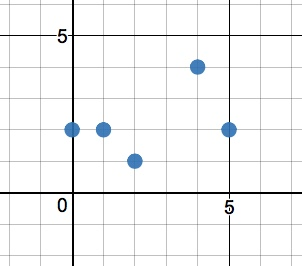
\includegraphics[width=0.35\textwidth]{discrete-domain-graph.jpeg}
    \end{figure}

    \item What is the range of this function modeling a bicycle wheel?
    \begin{figure}[!ht]
        \centering
        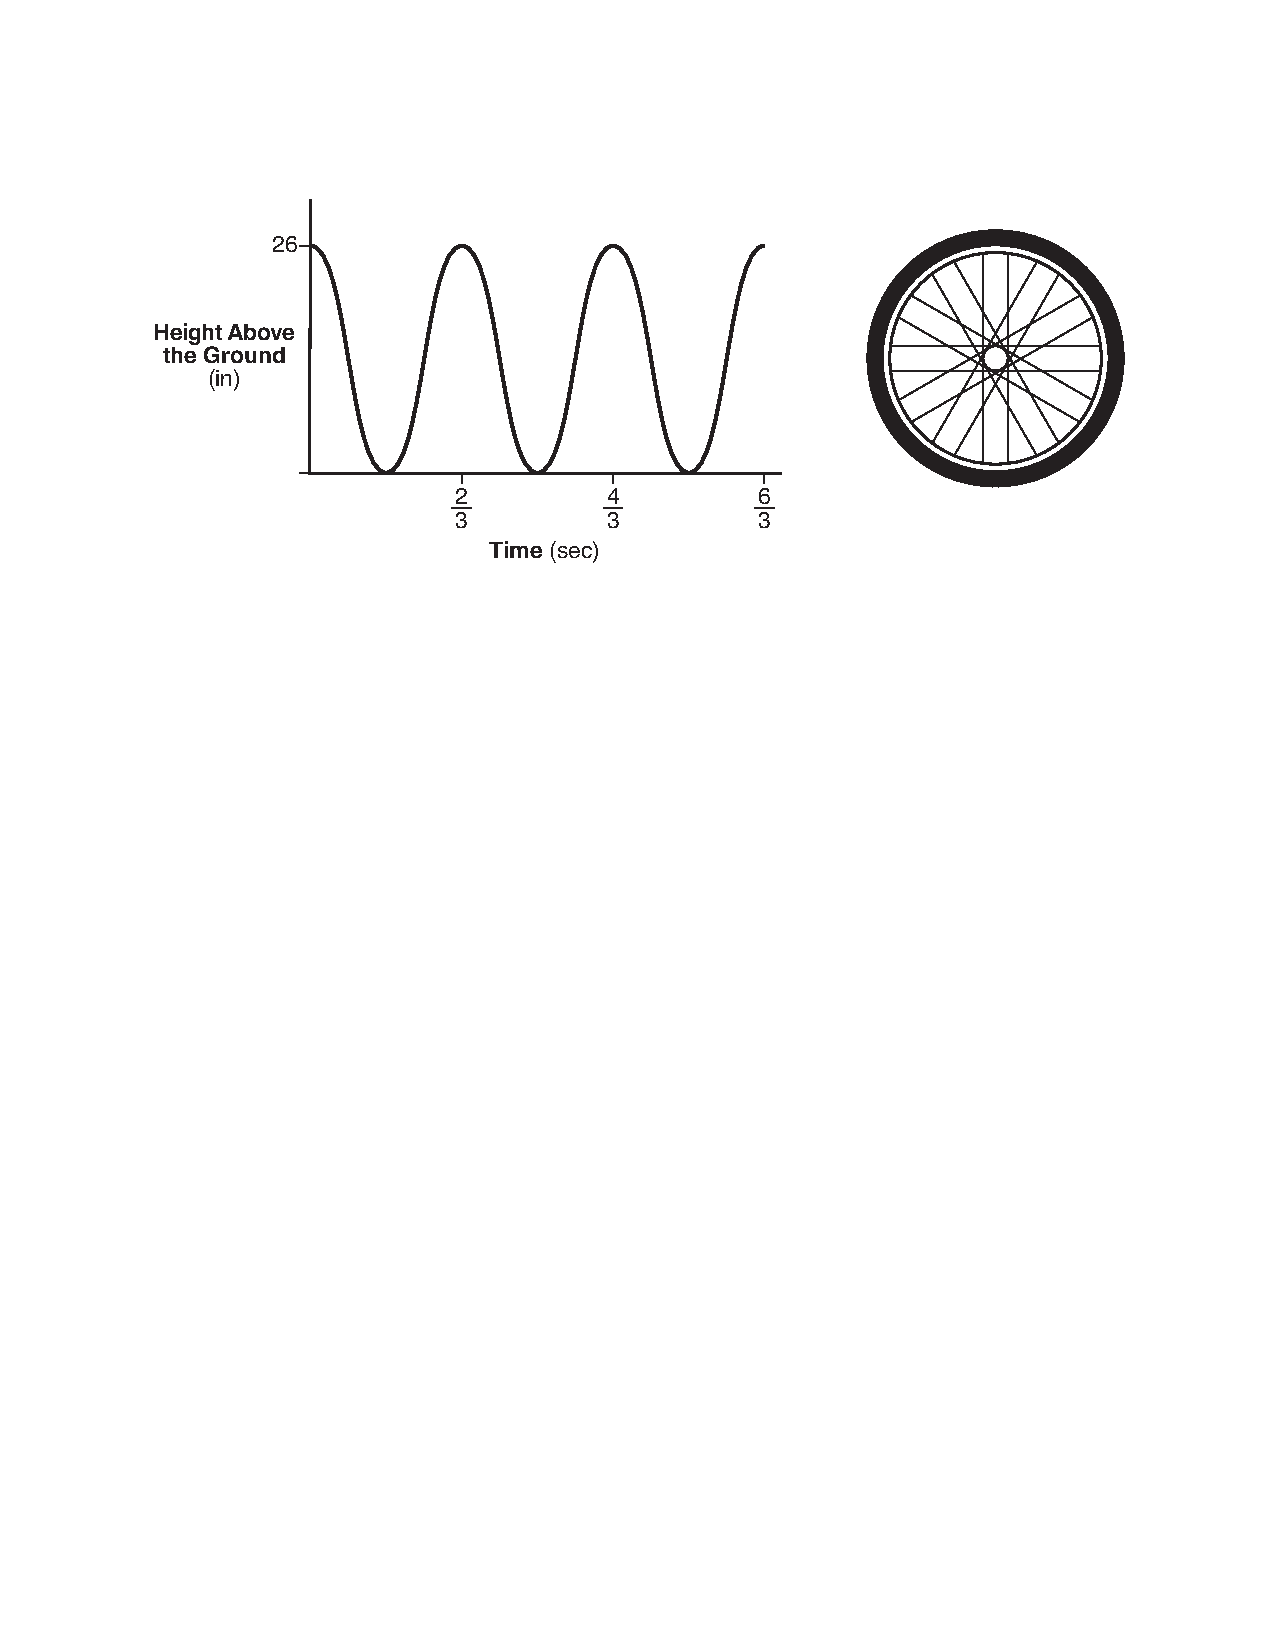
\includegraphics[width=0.70\textwidth]{sine-bike-wheel.pdf}
    \end{figure}
  \end{enumerate}
  }

\frame
{
  \frametitle{Function substitution \hspace{\stretch{1}} \alert{1.5}}
  Given $f(x)=3x+2$. What is $f(2x-1)$? \bigskip
    \begin{enumerate}
        \item Perform the substitution, putting $2x-1$ in parenthesis.\\*[20pt]
        \item Simplify, beginning each line with a leading equals sign if it is equal to the line above.\\*[40pt]
  \end{enumerate}
  }

  \section{1.4 Drui}
  \frame
  {
    \frametitle{GQ: How do we solve quadratic equations?}
    \framesubtitle{CCSS: HSF.IF.B.4 Interpret key features of functions and their graphs \hfill \alert{1.4 Tuesday 10 Sept}}

    \begin{block}{Do Now: Factoring}
    \begin{enumerate}
      \item Find the intercepts, axis of symmetry, and minimum point of the graph of the function $f(x)=(x-1)(x-5)$?
      \item Factor the function $g(x)=x^2-x-12$ to determine the features of its graph.
      \item Convert the function $h(x)=x^2+4x+3$ to the vertex form, $h(x)=a(x-h)^2+k$. Write down its vertex.
    \end{enumerate}
    \end{block}
    Lesson: Factoring, setting $=0$, checking solutions, $x-$ and $y-$intercepts, vertex, axis of symmetry
    \\ \bigskip
    Homework: Factoring practice, completing the square, graphing\\
    Skip around and do what you can by tomorrow
  }

  \section{1.5 Drui - Monday September 17}

  \frame
  {
    \frametitle{How do we graph quadratics?}
    \framesubtitle{CCSS: HSF.IF.B.4 Interpret key features of functions and their graphs \hspace{\stretch{1}} \alert{1.5}}

    \begin{block}{Consider the function $f(x)=-x^2+2x+3$}
    \begin{enumerate}
        \item Factor $f$ and state its zeros.
        \item Restate $f$ in vertex form. Write down the vertex as an ordered pair.
        \item Over what intervals is the function increasing, decreasing, and neither?
        \item If $f(x)$ represents the height of a diver over the domain $0 \leq x \leq 3$, interpret $f(0)$, the vertex, and $f(3)$
        \item What does the "slope" of the curve represent?
    \end{enumerate}
    Lesson: Example 18 p. 54
    \end{block}
  }


\section{1.6 Drui Tuesday September 18th, laptop cart D}
  \frame
  {
    \frametitle{How do we communicate mathematical results?}
    \framesubtitle{CCSS: MP.4 Model with mathematics \hspace{\stretch{1}} \alert{1.6}}

    \begin{block}{Technical skills needed to communicate mathematics}
    \begin{enumerate}
        \item Word processing: Microsoft Word and equation editor
        \item Computer calculators: Desmos; domain restriction, labeling
        \item Cloud storage: Dropbox
        \item Technical writing standards: MLA format (Purdue OWL)
        \item Writing style: declarative
        \item Assessment criteria: IB exploration criterion \emph{B: Mathematics Presentation}
    \end{enumerate}
    \end{block}
    Lesson: Shared folder structure, graph copy/paste, MLA template\\ \bigskip
    Homework: Pre-test
  }

\section{1.7 Drui Review Thursday September 20th}
  \frame
  {
    \frametitle{GQ: How do we simplify exponents?}
    \framesubtitle{CCSS: HSN.RN.A.2 Rewrite expressions involving radicals and rational exponents using the properties of exponents \hspace{\stretch{1}} \alert{1.7}}

    \begin{block}{Do Now: Exponent and radicals practice}
      \begin{enumerate}
      \item Exponent product, quotient, and power rules
      \item Fractional exponents
      \item Negative exponents
      \item Graphing exponential function
      \end{enumerate}
   \end{block}
    Lesson: Product, quotient, power rules, $\sqrt{x^4}$ \\ \bigskip
    Homework: Exponent and radicals practice
  }

\end{document}

\section{1.8 Unit exam September 24th}
  \frame
  {
    \frametitle{GQ: How do we use functions in algebra?}
    \framesubtitle{CCSS: HSF.IF.B.4 Interpret key features of functions and their graphs \hspace{\stretch{1}} \alert{1.8}}

  Exam \\ \bigskip
  Homework: Pre-test
  }
